
\chapter{Técnicas para detecção e reconstrução de oclusões parciais}
\label{cp:5_reconstrução}

Este capítulo possui como objetivo principal apresentar algumas técnicas para detecção e reconstrução de oclusões parciais em imagens de face. Todas as técnicas apresentadas neste capítulo são provenientes de uma revisão sistemática feita durante o desenvolvimento deste trabalho, esta RS encontra-se disponível no trabalho de \cite{Targino2018_wvc}. 


\section{Contextualização da literatura}

Durante a elaboração deste trabalho analisou-se uma grande quantidade de trabalhos relacionados, a depender de sua temática junto a identificação biométrica da face. Com iniciativas a lapidar as técnicas analisou-se alguns trabalhos relacionados com iniciativas a implementação das mesmas para comparações futuras. Dentre os trabalhos podemos perceber que o artigo de \citeonline{[11]lai2013robust} apresenta uma técnica para detecção da oclusão utilizando um estimador robusto com regressão linear, em que o mesmo analisa os pixels correspondentes no conjunto de treinamento e os classifica como não ocluídos, diante disso a imagem analisada é classificada de acordo com a classe com menor erro de reconstrução. Já \citeonline{[2]zhang2016face} utiliza sete Redes Neurais Convolutivas (do inglês: \textit{Convolutional Neural Network} (CNN)) para detecção da oclusão, dessas setes redes, três, duas e duas, são responsáveis por detectar respectivamente a cabeça, olhos e boca, utilizando a estratégia de \textit{Max-pooling} como processo de discretização e redução do número de parâmetros para entrada na rede. O primeiro nível da  CNN é  responsável por rejeitar rapidamente a maioria das janelas de detecção, já o segundo nível julga se as janelas restantes são pontos faciais ou não.

Enquanto \citeonline{[4]wei2014dynamic} apresenta a estratégia DICW, esta divide a imagem da face em $P$ partes e logo em seguida analisa a diferença das tonalidades entre as partes a partir da manipulação de séries temporais, e logo após aplica distância euclidiana para analisar a presença de possíveis oclusões nas partes da imagem. Já \citeonline{[12]sharma2013efficient} detecta a parte ocluída por meio da aplicação de um limiar na imagem em escala de cinza, com isso obtendo a máscara de oclusão.
 
 


A metodologia clássica para tratar o reconhecimento biométrico baseado em imagens de faces ocluídas consiste em encontrar características ou classificadores tolerantes à ruído. Vários trabalhos têm demonstrado que os algoritmos locais são menos sensíveis a oclusões parciais. Buscando aplicar tais algoritmos, \citeonline{PenioPenev_1996} propuseram Análise de Características Locais para extração de características usando estatísticas de segunda ordem. Já \citeonline{Martinez_2002} propôs uma abordagem que consiste em dividir  a imagem da face ocluída em $k$ regiões locais, sendo possível segmentar a região parcialmente ocluída por meio de um modelo probabilístico. Além disso, foi proposto uma ponderação para regiões locais a fim de fornecer robustez em problemas que envolvem variação de expressão. Uma extensão do trabalho de \citeonline{Martinez_2002} foi proposta por \citeonline{Tan_2005}, em que o mesmo utilizou Mapas Auto-Organizáveis (do inglês: \textit{Self Organizing Maps} - SOM) para apreender o subespaço ao invés de usar Gaussianas ou Mistura de Gaussianas como modelo probabilístico.

Paralelamente \citeonline{Jongsun_2005} propôs um método chamado Analises de Componentes Independentes baseado em Saliências Locais, o qual emprega  informação de saliências locais na extração dos componentes independentes. Enquanto \citeonline{Zhang_2007} utilizou a divergência de Kullback-Leibler  para estimar a distribuição de probabilidade de oclusões no espaço de característica, de modo a melhorar o método LGBPHS (do inglês: \textit{Local Gabor Binary Pattern Histogram Sequence}) para a detecção da oclusão na imagem de face.



Em outro ângulo \citeonline{[20]shermina2012recognition} dividem a imagem da face em $B$ blocos e aplicam a técnica de correspondência por blocos para detecção da parte ocluída, utilizando uma máscara de tamanho ($3 \times 3$).  Enquanto  \citeonline{[22]chiang2011recognizing} utilizam o método Descoberta Iterativa da Face (do inglês: \textit{Iterative Face Recovery} - IFR), este método sendo responsável por criar conexões triangulares entre os pontos de referência da face, e com isso facilitar o processo de detecção da oclusão .




Em \citeonline{[38]tan2005recognizing} aplicou-se o algoritmo SOM para projetar a relação topológica da face e assim localizar a região ocluída na imagem da face com o auxílio do KNN\nomenclature{KNN}{k-Nearest Neighbors} como classificador. Em contrapartida \citeonline{[36]huang2012subface} utilizam Modelos Ocultos de Markok (do inglês: \textit{Hidden Markov Models} - HMM), com esta técnica sendo possível identificar os componentes faciais por meio de uma gramática facial. Nessa técnica foi possível aplicar o Modelo de Oclusão Universal (do inglês: \textit{Universal Occlusion Model} - UOM) \nomenclature{UOM}{Universal Occlusion Model} para identificar a localização da oclusão, como também qual componente facial ela está ocluindo. O trabalho de \citeonline{[34]zhang2006robust} apresenta a Memória de Kernel Associativo( do inglês: \textit{Kernel Associative Memory} - KAM) com multi escala de transformação de Gabor. Já \citeonline{[31]su2009multi} apresentam a técnica Alinhamento de Faces Multi-visões (do inglês: \textit{Multi View Face Alignment }- MVFA) sendo responsável por alinhar a face e identificar pontos de oclusão, entretanto essa abordagem apresenta-se pouco voltada a oclusão, tendo maior ênfase para o alinhamento da face a partir das variações de pose.

Enquanto para o contexto de reconstrução da faces temos alguns trabalhos que tornaram-se essenciais para a realização deste trabalho. Os quais são descritos com maiores detalhes logo em seguida.




Dentre alguns trabalhos dispostos na literatura existem alguns que se destacam perante os demais. Como o trabalho de \citeonline{[25]deng2011graph} que utiliza um grafo espectral baseado na ideia de reconstrução da imagem, em que o algoritmo cria uma matriz esparsa para representar a parte parcialmente ocluída da imagem e com isso realizar a consulta no conjunto de treinamento, logo em seguida aplicando a topologia do grafo de Poisson na imagem do treinamento com maior similaridade para descoberta dos pixels ocluídos por meio da resolução de um sistema linear.

Sobre outra perspectiva  \citeonline{[37]hosoi2012restoring} apresentou a técnica FW-PCA(do inglês: \textit{Fast Weighted - Principal Componente Analysis}), nesta técnica a imagem da face é reconstruída a partir do espaço de faces, a qual realiza a atualização a cada iteração, gerando uma máscara de oclusão robusta, a qual  consequentemente possibilita melhores imagens reconstruídas. \citeonline{[34]zhang2006robust} aplicam modelos de KAM baseadas em transformações de Gabor, em que as imagens de face são decompostas em representações multi-escala pela transformação de Gabor e depois modelada pelas KAM para sua posterior reconstrução. 

Em outro contexto, \citeonline{[17]alyuz2012robust} e \citeonline{[14]alyuz20133} utilizaram a técnica Ponto Iterativo mais Próximo (do inglês: \textit{Iterative Closest Point} - ICP) \nomenclature{ICP}{Iterative Closest Point} para detecção da oclusão, e para reconstrução da face aplicaram \textit{Gappy} PCA com iniciativas a encontrarem melhores coeficientes de combinação linear com redução do erro de reconstrução, em que esses coeficientes passaram pelo processo de minimização do gradiente. Paralelamente, \citeonline{[1]bellil2016gappy} aplicam comparações de coeficientes Wavelet da imagem ocluída com todas as imagens do conjunto de treinamento, e para a tarefa de reconstrução da face utilizaram a técnica GWNN (do inglês: Gappy Wavelet Neural Network). 

Enquanto \citeonline{min2011improving} aplicaram um modelo que procura por partes ocluídas na imagem facial, de modo que esse modelo foi construído fazendo uso das técnicas Gabor Wavelet para análise da textura, PCA para projeção das faces no espaço de faces e o classificador SVM para classificação dos pixels ocluídos a cada iteração. Logo após esse processo são realizados os testes de reconhecimento com as imagens resultantes. \citeonline{storer2009fast} propôs o FRPCA (do inglês: \textit{Fast Robust PCA}), o qual detecta os pixels efetivos usando uma quantidade $K$ de pequenos espaços de faces computados pela seleção de $P$ pixels selecionados aleatoriamente, de modo que o conjunto de treinamento e teste fazem uso do processo de detecção dos pixels efetivos. A base dessa técnica realiza o armazenamento de todos os pequenos subespaços computados do conjunto de  treinamento para a cada iteração incrementar o número de pixels efetivos.


Já em  \citeonline{Fidler_2006} foi proposto a combinação de métodos baseados em subespaço, como Análise de Componentes Principais (do inglês: Principal component Analysis - PCA), com métodos que visam a discriminação, como Análise de Discriminante Linear (do inglês: \textit{Linear Discriminant Analysis} - LDA), objetivando melhor reconstrução das imagens de face.  Por outro lado, \citeonline{Jia_2009} propôs emprego de Máquinas de Vetores Suporte  em cenários em que a oclusão pode ocorrer em ambos os conjuntos de treinamento e teste. Neste caso, problema de oclusão foi tratado como um problema de reconstrução e a classificação foi realizada de acordo com o erro de reconstrução obtido para a imagem de teste. 


Paralelamente \citeonline{[20]shermina2012recognition,[22]chiang2011recognizing} utilizam como método de reconstrução PCA, utilizando os \textit{Eigenfaces} com maiores autovalores para reconstruir as imagens parcialmente ocluídas. Enquanto \citeonline{[12]sharma2013efficient} utilizam filtros de Gabor com oito variações de ângulos gerando oito conjuntos de treinamento, utilizando a técnica PCA para projetar oito subespaços referentes aos respectivos conjuntos de treinamento. Dessa forma reconstruindo as imagens e utilizando o espaço de face que apresentou melhores níveis de reconstrução para a tarefa de classificação.


Sobre a perspectiva de detecção dos pontos faciais reconstrução da face  no trabalho \citeonline{hwang2000face} é proposto um método para reconstruir faces parcialmente ocluídas por meio da seleção manual de alguns pontos característicos na região facial, sendo baseado na forma da face. Dessa forma sendo possível estimar os coeficientes de combinação linear das faces de treinamento por meio das informações obtidas com o modelo.	
 




\section{Técnicas para detecção de oclusões parciais}
Dos trabalhos dispostos na literatura para detecção da oclusão neste trabalho foram utilizadas três técnicas, as quais são descritas em maiores detalhes logo abaixo:

\subsection{Skin Tone}

A técnica \textit{Skin Tone} \cite{cheddad2009skin} foi a primeira técnica a ser utilizada para detecção da oclusão na imagem de face, essa técnica em sua ideia original abordada na subseção \ref{sub:skin} é utilizada para detecção da face, entretanto também pode ser utilizada para detecção da oclusão. Após a aplicação da técnica Viola-Jones para detecção da face, utilizamos a técnica \textit{Skin Tone} para análise de seu comportamento perante a tarefa de detecção da parte ocluída. Para detecção da oclusão com essa técnica é obrigatório que a imagem de consulta esteja em RGB.

Durante os experimentos percebeu-se sensibilidade dessa técnica junto a detecção dos pixels ocluídos, quando apresentadas a contextos não controlados, dessa forma possibilitando baixa performance de segmentação dos pixels ocluídos com tonalidades próximas a tonalidade da pele, assim como também oclusões com variações de iluminação. Consequentemente gerando uma máscara de oclusão com perda de informações.

Por meio do algoritmo \ref{alg:algoritmo_skin} podemos perceber o funcionamento dessa técnica perante a tarefa de construção da máscara de oclusão.

\begin{algorithm}[H]
\caption{Skin Tone}
\label{alg:algoritmo_skin}
\begin{algorithmic}[1]

%\Procedure{Skin Color}{}
\State $im \gets imagem$
\State $[l,c,a] \gets size(im)$
%\for{i \gets 0 : 1}
%\State $bw = zeros(l,c)$
\For{$i = 1$ to $l$}
	\For{$j = 1$ to $c$}
      \State $I(l,c) \gets im(l,c,1)*0.298 + im(l,c,2)*0.587 + im(l,c,3)*0.140$
     
	\EndFor
\EndFor

\For{$i = 1$ to $l$}
	\For{$j = 1$ to $c$}
      \State $\hat{I}(l,c) = max( im (l,c,2), im(l,c,3))  $ 
     \EndFor
\EndFor
\State $E = I - \hat{I}$
     
\For{$i = 1$ to $l$}
	\For{$j = 1$ to $c$}
     
     \If {$E(l,c) <= 0.0251$  \&  $E(l,c) >= 0.1177$ }
            \State $mascara(l,c) = 1$
      \Else
      		\State $mascara(l,c) = 0$
             
    \EndIf
      
	\EndFor
\EndFor
\State $retorne$ $mascara$

%\EndProcedure
\end{algorithmic}
\source{Jonas Mendonça Targino, 2018. Baseado no trabalho de \cite{cheddad2009skin} }
\end{algorithm}





\subsection{Limiarização}

Essa técnica utilizada por \citeonline{[12]sharma2013efficient} para detecção da parte ocluída, tendo como princípio a aplicação de um limiar em uma imagem parcialmente ocluída em escala de cinza para construir a máscara de oclusão da imagem. 
Neste trabalho a partir de inúmeros experimentos verificou-se que o limiar igual a 78 seria um bom limiar de aplicação da técnica para cenários controlados. Entretanto, essa técnica ao ser apresentada a imagens de face com variações de iluminação e oclusão apresentou resultados desfavoráveis de segmentação da parte ocluída na imagem da face. A máscara de oclusão dessa técnica pode ser gerada conforme a equação \ref{eq:bin_limiar}.

\begin{equation}
\label{eq:bin_limiar}
I_{Binaria} = \left\{\begin{matrix}
0 &  \textrm{se imagem(x,y)} \leq \textrm{limiar} \\ 
1 & \textrm{caso contrario}
\end{matrix}\right.
\end{equation}

Inicialmente nos experimentos foi utilizada essa técnica para tentar detectar a oclusão, entretanto a mesma apresentou queda de performance quando submetida a detecção de oclusões com tonalidades próximas a cores da pele humana, como também oclusões com iluminações. Essa técnica apresentou melhores segmentações da parte parcialmente ocluída do que a técnica \textit{Skin Tone}.


\subsection{Algoritmo de correspondência dos blocos}

A técnica Algoritmo de Correspondência dos blocos (do inglês: \textit{Block Matching Algorithm} - BMA),  proposta por \cite{[20]shermina2012recognition} é responsável por realizar a divisão da imagem $I$ em $K$ blocos de tamanho (N $\times$ N). Na equação \ref{eq:bma} é representada a estrutura da imagem $I$ após sua divisão em $K$ blocos.

\begin{equation}
\label{eq:bma}
I = \{Ib_1, Ib_2,.....,Ib_{K} \}
\end{equation}

No BMA divide-se a imagem em blocos de tamanhos similares que são utilizados para detectar a oclusão na imagem da face. Como estratégia de comparação entre os blocos com vistas a detectar a parte ocluída e não ocluída é utilizada a distância Euclidiana, a qual é utilizada para analisar a similaridade entre as imagens dos blocos.

Para análise de similaridade e correspondência entre os blocos compara-se cada imagem ocluída (imagem de consulta), com uma imagem presente na base de dados. Visto que uma imagem de consulta $q$ foi dividida em $K$ blocos descritos conforme a  equação \ref{eq:imagem_consulta}.

\begin{equation}
\label{eq:imagem_consulta}
I = \{qb_1, qb_2,.....,qb_{K} \}
\end{equation}

Então comparamos cada bloco da imagem de consulta e a imagem presente no banco de dados, essa comparação sendo possível com auxílio das métricas da distância Euclidiana. Como descrito na equação \ref{eq:dist_euclidiana}.

\begin{equation}
\label{eq:dist_euclidiana}
Ed_a = \sqrt{\sum (Ib_a - qb_a)}^2
\end{equation}



Podemos visualizar com o auxílio da figura \ref{fig:esquema_bma} o processo de detecção da oclusão por meio da técnica BMA.


\begin{figure}[H]
\centering
\caption{Esquema do BMA}
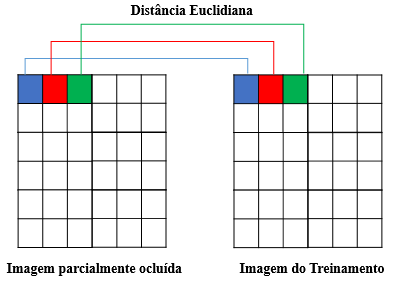
\includegraphics[scale = 0.8]{imgs/bma.png}
\label{fig:esquema_bma}
\source{Jonas Mendonça Targino, 2018}
\end{figure}


Em que $a$ é o número de blocos das imagens. Após o cálculo da distância Euclidiana aplica-se um limiar para remover a oclusão. Na figura \ref{fig:detec_blocos} apresenta-se na primeira linha imagens com oclusões parciais, e na segunda linha imagens com suas respectivas oclusões detectadas por meio de uma máscara de tamanho (2 $\times$ 2).

\begin{figure}[H]
\centering
\caption{Detecção da parte ocluída com a técnica de detecção por blocos}
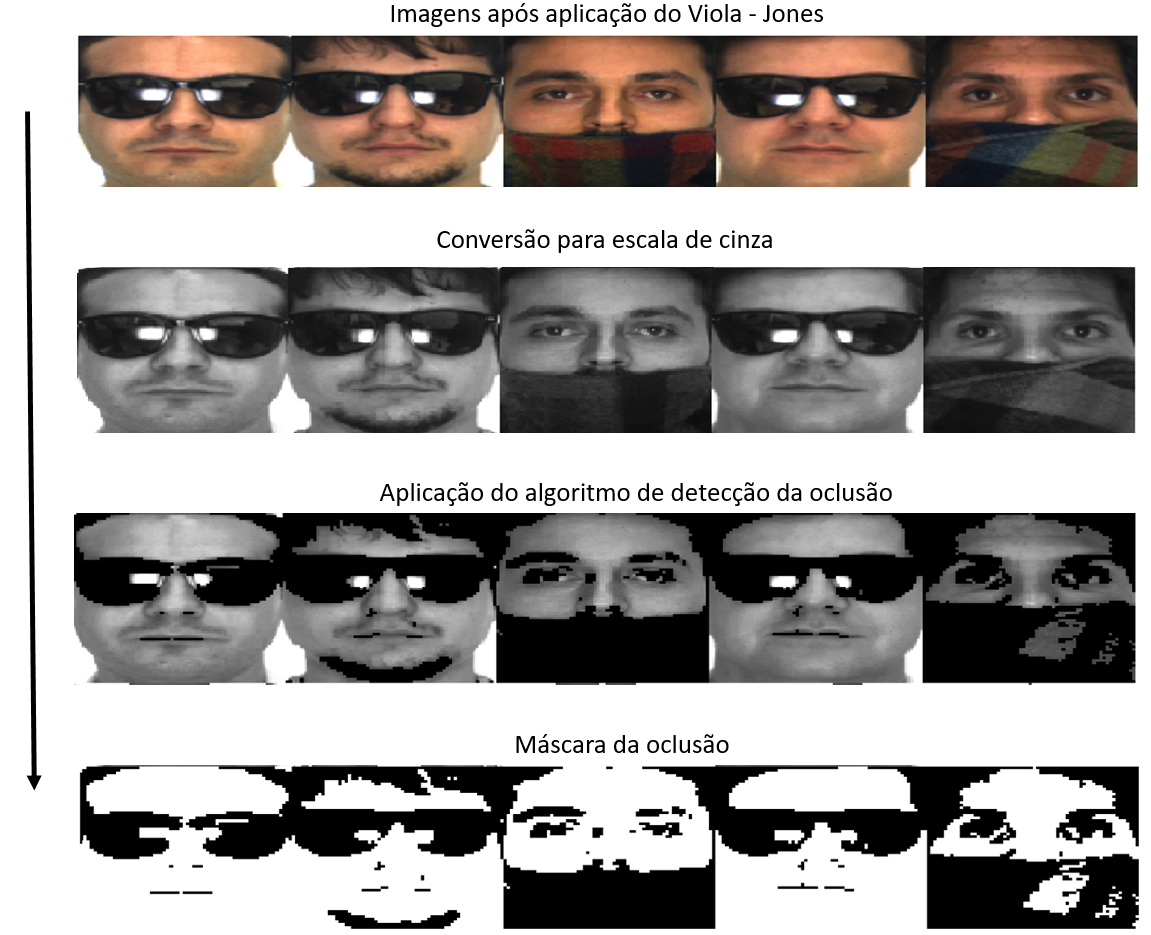
\includegraphics[scale = 0.40]{imgs3/deteccoes}
\source{Jonas Mendonça Targino, 2018. Imagens de faces obtidas após aplicação do Viola-Jones na base AR \cite{martinez1998ar}}
\label{fig:detec_blocos}
\end{figure}


\section{Técnicas de reconstrução baseadas em subespaço}


As técnicas de reconstrução baseadas em subespaço possuem como princípio fundamental a projeção das imagens em um espaço de faces. Na figura \ref{fig:pca1} é possível visualizar uma face de entrada sendo projetada em um espaço de faces contendo dois \textit{eigenfaces}. O DFFS representa uma métrica de distância daquela imagem para espaço de faces.



\begin{figure}[H]
\centering
\caption{Projeção de uma imagem no subespaço}
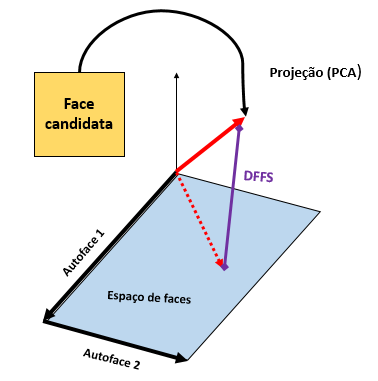
\includegraphics[scale = 0.75]{imgs/pca1.png}
\source{Jonas Mendonça Targino, 2018. Adaptado de \citeonline{chollet2007some}}
\label{fig:pca1}
\end{figure}

Entretanto ao trabalharmos com faces parcialmente ocluídas, a modelagem segue a mesma estrutura, com diferencial que a imagem de entrada possui pixels pretos na parte ocluída, com iniciativas que aqueles pixels não influenciem erroneamente na projeção da imagem facial. Na figura \ref{fig:pca2} é possível visualizar a forma de projeção de uma imagem parcialmente ocluída no subespaço.

\begin{figure}[H]
\centering
\caption{Projeção de uma imagem parcialmente ocluída no subespaço}
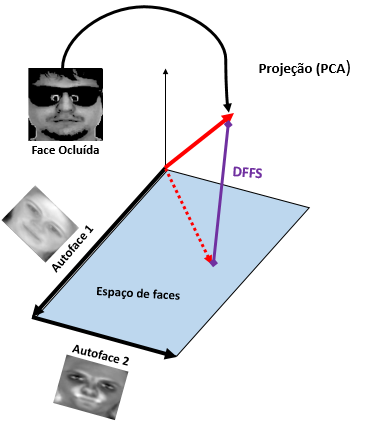
\includegraphics[scale = 0.75]{imgs/pca2.png}
\source{Jonas Mendonça Targino, 2018}
\label{fig:pca2}
\end{figure}



\subsection{Eigenfaces}

\textit{Eigenfaces} proposto por \citeonline{turk1991face} é uma técnica para reconstrução facial, sendo a primeira a ser vista como um sucesso, essa técnica utiliza um conjunto de autovetores que são projeções escuras de faces, em que essas projeções quando combinadas linearmente representam cada imagem do conjunto de faces. O \textit{Eigenfaces} utiliza princípios do PCA com iniciativas a projetar as imagens em um espaço de características de baixa dimensão, partindo da ideia que a imagem na alta dimensão pode ser descrita por variáveis correlacionadas, sendo necessário poucas dimensões para representar a maior parte da informação da imagem, nesse meio termo atuando o PCA, de modo a encontrar as direções com maior concentração dos dados, denominados componentes principais.

No \textit{Eigenfaces} todas as \textit{M} imagens de treinamento de face são de dimensões ($L \times C$), cada uma dessas imagens deve ser transformada em uma imagem com dimensões $F = (L\cdot C \times 1)$. Logo em seguida são representadas por uma matriz $\Gamma$, esta matriz contém \textit{M} imagens de treinamento \textit{$ \Gamma = \{ I_1,I_2,I_3...I_M \}$}. 


$I_i = \begin{bmatrix}
 a_{11}  & ...  & a_{1C}\\ 
 : & : & :\\ 
 a_{L1}& ... &a_{LC} 
\end{bmatrix}(L \times C)
\rightarrow 
\begin{bmatrix}
a_{11} \\ 
 :\\ 
 a_{L1}\\
:\\
a_{1C}\\
:\\
a_{LC} 
 
\end{bmatrix} (F \times 1) = \Gamma_i $

Tendo um conjunto de \textit{M} imagens de treinamento a equação \ref{eq:mediaEig} apresenta o  cálculo da imagem média das faces. Enquanto a figura \ref{fig:imMedia} ilustra a forma de uma imagem média obtida de um conjunto de treinamento.

\begin{equation}
\mu = \frac{1}{M} \sum_{i=1}^{M} \Gamma_i 
\label{eq:mediaEig}
\end{equation}


\begin{figure}[H]
\centering
\caption{Exemplo de formação da imagem média dado um conjunto de imagens}
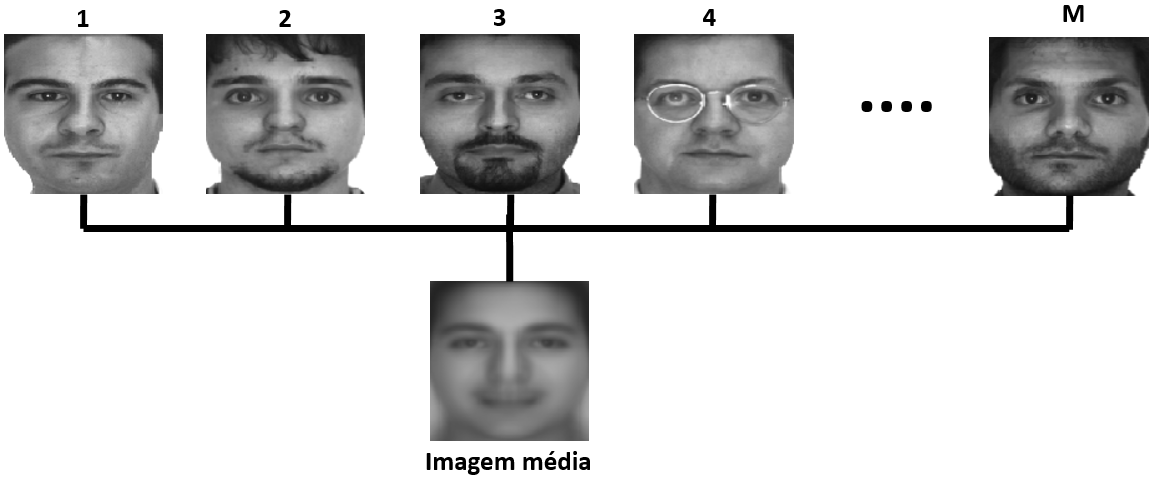
\includegraphics[scale = 0.50]{imgs3/imMedia.png}
\source{Jonas Mendonça Targino, 2018. Imagens de faces obtidas da base AR \cite{martinez1998ar}}
\label{fig:imMedia}
\end{figure}




Logo após a imagem média das faces ser calculada, faz-se necessário calcular a dissimilaridade entre cada imagem da face $\Gamma_i$ e a imagem média $\mu$, essa proposta de subtração de cada imagem pela imagem média faz-se necessária para distinguir as características de cada face e com isso remover as informações em comum. É possível visualizar o cálculo da matriz de dissimilaridade $A$ conforme a equação \ref{eq:teta}.

\begin{equation}
\Theta_i = \Gamma _i - \mu, \textit{sendo A} = [\Theta_1,\Theta_2,...\Theta_n]
\label{eq:teta}
\end{equation}

Com a matriz $A$ encontrada, é possível extrair os autovetores e autovalores da matriz de covariância das imagens de treinamento, a matriz de covariância é obtida como segue na equação \ref{eq:covariancia}.

\begin{equation}
C = A \cdot A'
\label{eq:covariancia}
\end{equation}

Entretanto, encontrar os autovalores e autovetores é uma tarefa muito custosa para o tamanho das imagens utilizadas, visto que a matriz de covariância será da ordem ($F \times F$), assim uma maneira simplificada foi adotada por \citeonline{turk1991face}, em que dada a matriz de covariância podemos representá-la por meio do produto entre $A'\cdot A$, gerando uma matriz ($M \times M$) que é inúmeras vezes menor. Após essa mudança de operações para adquirir a matriz de covariância e seus subsequentes autovetores é possível obter os \textit{Eigenfaces} a partir da multiplicação da matriz $A$ pelos autovetores da matriz $C$ representados por $\beta$, como apresenta a equação \ref{eq:autoVet}. Com base na fórmula podemos perceber redução do número de \textit{Eigenfaces} para um valor $k$, esse valor significa que esses $k$ \textit{Eigenfaces} são os mais representativos do conjunto.

\begin{equation}
\begin{matrix}
\Phi = A \cdot \beta  \\
\textrm{dessa forma } \Phi \textrm{ possui } m \textrm{ Eigenfaces} \\
\Phi  = [v_{1},v_{2} \cdots v_m] \\
\textrm{logo selecionamos os } k \textrm{ melhores Eigenfaces}\\
\Phi = [v_{1},v_{2} \cdots v_k] 
\end{matrix}
\label{eq:autoVet}
\end{equation}

Após encontrados os \textit{Eigenfaces} representados por $\Phi$, temos a representação das imagens da face em formas de sombras como podemos ver na figura \ref{fig:eigenfaces}. 

\begin{figure}[H]
\centering
\caption{Exemplos de 10 \textit{eigenfaces} da base de dados \textit{AR}}
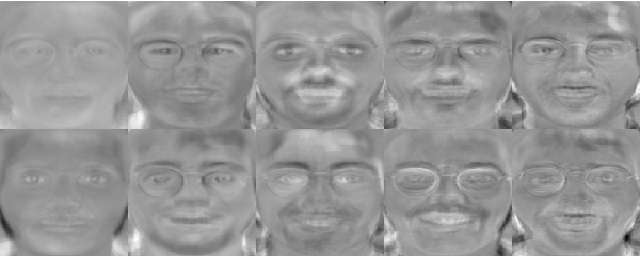
\includegraphics[scale = 0.90]{imgs/eigenfaces.png}
\source{Jonas Mendonça Targino, 2018}
\label{fig:eigenfaces}
\end{figure}

Após esse passo devemos encontrar os coeficientes de combinação linear $y$ que podem serem obtidos por meio da equação \ref{eq:yi}, de modo que $\Upsilon$ e $v_i$ representam respectivamente a imagem de consulta e o \textit{Eigenface}.

\begin{equation}
y_i = (\Upsilon - \mu) \cdot v_i
\label{eq:yi}
\end{equation}

Ao encontrarmos os coeficientes de combinação e os \textit{Eigenfaces} podemos reconstruir uma imagem de consulta de acordo com a fórmula \ref{eq:recpca}. Nessa fórmula $K$ representa os $K$ melhores \textit{Eigenfaces} selecionados.

\begin{equation}
\hat{\Upsilon} = \mu + \sum_{i=1}^{K}y_i \cdot v_i 
\label{eq:recpca}
\end{equation}


 Ao realizarmos a reconstrução da imagem de face e projetarmos essa imagem no espaço de faces podemos obter sua distância para o espaço de faces (do inglês: \textit{Distance from face space} - DFFS), esta medida sendo responsável por avaliar se uma dada imagem pode representar uma face ou não, mediante análise da distância entre o espaço de faces e tal imagem. A equação para obtenção do DFFS pode ser vista na equação \ref{eq:normaE}.


\begin{equation}
DFFS = \left| -\Upsilon + \mu + \sum_{i=1}^{K}y_i \cdot v_i \right|
\label{eq:normaE}
\end{equation}

É importante notar que quanto maior o DFFS de uma imagem de consulta maior a chance daquela imagem estar ocluída, de modo que faces ocluídas tendem a não combinar linearmente com \textit{Eigenfaces} calculados com exemplos de imagens não ocluídas. Com isso, quando uma imagem é reconstruída a partir de \textit{Eigenfaces} a parte ocluída tende a ficar mais evidenciada. 

A parte ocluída é detectada por meio de um limiar escolhido empiricamente analisando a diferença entre o pixel original e o pixel reconstruído. Assim sendo possível remover a suposta parte ocluída a partir do limiar, vale ressaltar que a escolha do limiar pode não ser tão preciso, isso fica a depender da tonalidade da oclusão e iluminação presente na imagem. 

De modo a tentar realçar a região ocluída e minimizar a chance de um limiar não ser tão preciso, uma das motivações de aplicação para um bom realce da máscara de oclusão é aplicar filtros morfológicos, de modo que os filtros preparam a imagem para a fase de reconstrução da imagem. Esses filtros são aplicados em duas fases, sendo a primeira responsável por preencher os espaços vazios deixados pela eliminação das partes ocluídas, e a segunda descartar pequenas regiões que não aparentam ser regiões ocluídas, por exemplo regiões que possuem área ocluída muito pequena, como as regiões próximas ao nariz e a boca. Podemos ver a ilustração de uma problemática como essa na figura \ref{fig:mascara}.


\begin{figure}[H]
\centering
\caption{Máscara de remoção de oclusão}
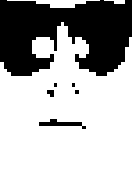
\includegraphics[scale = 0.62]{imgs/mascara.png}
\source{Jonas Mendonça Targino, 2018}
\label{fig:mascara}
\end{figure}




\subsection{Gappy PCA}
Após a detecção da oclusão com \textit{Eigenfaces} a imagem da face deve passar pelo processo de reconstrução. Uma das estratégias de reconstrução da imagem da face é o GPCA (do inglês: \textit{Gappy Principal Component Analysis}) \cite{colombo2009gappy}. Essa estratégia tem como base um conjunto de imagens de faces ocluídas \{$\Upsilon_1,\Upsilon_2, \cdots ,\Upsilon_N$\}, em que cada face possui um vetor \textit{y} de coeficientes, e a tarefa principal dessa estratégia é encontrar um vetor de $y$ que minimize o erro de reconstrução da imagem. Assim, uma imagem de face com oclusão pode ser restaurada com o auxílio da combinação linear entre um vetor de coeficientes \textit{y} com os \textit{Eigenfaces}, conforme a equação \ref{eq:erroDffs}. Nesta equação a variável $\mu$ e $K$ representam respectivamente a imagem média e o número de \textit{Eigenfaces} selecionados.


\begin{equation}
\Upsilon + e = \mu + \sum_{i=1}^{K}y_i \cdot v_i
\label{eq:erroDffs}
\end{equation}

Para calcular os coeficientes $y_i$, o DFFS  deve ser minimizado. Contudo, o DFFS é calculado a partir das imagens com oclusões parciais. Para realizar a reconstrução da imagem faz-se necessário calcular o produto \textit{gappy} dado por $(u,v)_z$, conforme equação \ref{eq:produtogappy}, em que o vetor \textit{z} é um vetor binário, contendo 0 caso a imagem $\Upsilon$ na posição $i$ for 0, ou seja, a oclusão foi removida na fase de detecção da oclusão, caso contrário $z_i$ = 1. De acordo com a equação \ref{eq:produtogappy} os termos $u_i$ e $v_i$ são os \textit{Eigenfaces}, e \textit{d} é a quantidade de pixels da imagem.


\begin{equation}
(u,v)_z = \sum_{i=1}^{d}u_i \cdot v_i \cdot z_i
\label{eq:produtogappy}
\end{equation}

Conforme mencionado os coeficientes $y_i$ são definidos de modo a minimizar o $\left \| e \right \|^2_z$, conforme a equação \ref{eq:minDFFS}.

\begin{equation}
\left \| e \right \|^2_z = \left \| - \Upsilon + \mu + \sum_{i=1}^{K}y_iv_i \right \|^2_z = \left \|    \Upsilon - \mu \right \|^2_z - 2\sum_{i=1}^{K}\sum_{j=1}^{K}y_iy_j(v_j,v_i)_z
\label{eq:minDFFS}
\end{equation}

Após o cálculo da derivada de $\left \| e \right \|^2_z$ em relação a $y_i$, considerando as derivadas parciais nulas, temos a equação \ref{eq:derivadayi}.

\begin{equation}
 \frac{\partial \left \| e \right \|^2_z}{\partial y_i} = -2(\Upsilon- \mu,v_i)_z + 2 \sum_{j=1}^{K}y_j(v_j,v_i)_z, \textit{para cada i em \{1,2,...K\}}
 \label{eq:derivadayi}
\end{equation}

Após os coeficientes $y_i$ encontrados por meio da minimização da equação \ref{eq:derivadayi}, é possível reconstruir a imagem com o auxílio da equação \ref{eq:recGPCA}.

\begin{equation}
\hat{\Upsilon} =  \mu + \sum_{i=1}^{K}y_i \cdot v_i
\label{eq:recGPCA}
\end{equation}




\subsection{Asymmetrical PCA}
\label{sub:apca}



 Análise dos componentes principais Assimétricos (do inglês: \textit{Asymmetrical Principal Component Analysis} -APCA) \nomenclature{APCA}{Asymmetrical principal component analysis} proposto por \citeonline{soderstrom2011asymmetrical} baseado no PCA \citeonline{jolliffe2002principal}. Com a técnica APCA é possível reconstruir regiões com oclusões parciais em imagens de face levando em consideração as regiões não ocluídas, de tal modo que a intensidade dos pixels das regiões não ocluídas é utilizada para estimar as regiões com oclusões parciais. A ideia principal do APCA surge a partir da criação de dois autovetores, um a partir dos pixels não ocluídos da imagem ocluída em que os vetores são ortogonais entre si e o outro, chamado de pseudo autovetor, ou autovetor falso, sendo construído a partir das imagens ocluídas. Dada a imagem $\Upsilon$, podemos representar a parte não ocluída de $\Upsilon$ como $\Upsilon^{no}$. De modo que $\Upsilon^{no}$ é modelado em um espaço vetorial $\Phi^{no} = \{ \phi _1^{no}, \phi _2^{no}, \phi _3^{no},...,\phi _N^{no} \}$, a equação \ref{eq:fino} apresenta a função responsável pelo mapeamento, em que $\beta_{ij}^{no}$ são os autovetores da matriz de covariância  A = \{ $(\Upsilon_i^{no} - \Upsilon _{\underline{o}}^{no})^T (\Upsilon_j^{no} - \Upsilon _{\underline{o}}^{no})  $ \} e $\Upsilon _{\underline{o}}^{no}$ é a média das regiões não ocluídas, o cálculo da média é apresentado na equação \ref{eq:imMedia}.

\begin{equation}
 \Phi^{no} = \sum_{i}\beta_{ij}^{no}(\Upsilon_{i}^{no} - \Upsilon_{\underline{o}}^{no}) 
\label{eq:fino}
\end{equation}

\begin{equation}
\Upsilon _{\underline{o}}^{no} = \frac{1}{n} \sum _{j=1}^{K} (\Upsilon_j^{no})
\label{eq:imMedia}
\end{equation}

Os valores dos autovetores das partes não ocluídas são utilizados para torná-los ortogonais, enquanto as partes ocluídas são modeladas a partir das tonalidades dos pixels das partes não ocluídas. Com isso, o pseudo autovetor pode ser construído conforme apresenta a equação \ref{eq:fiP}, em que $\Upsilon_i$ é a imagem original (face com oclusão) e $\Upsilon_{\underline{o}}$ é a média das imagens originais.

\begin{equation}
 \Phi_j^{P} = \sum_{i}\beta_{ij}^{no}(\Upsilon_{i} - \Upsilon_{\underline{o}}) 
\label{eq:fiP}
\end{equation}

A projeção é usada para extrair coeficientes $\{y_j^{no} \}$ do autovetor $\Phi _j^{no}$, conforme apresentado na equação \ref{eq:alfaNO}.

\begin{equation}
y_j^{no} = (\Upsilon_{i}^{no} - \Upsilon_{\underline{o}}^{no})^T \Phi _j^{no}
\label{eq:alfaNO}
\end{equation}

Ao final, podemos reconstruir a imagem utilizando a equação \ref{eq:recIM}, em que \textit{K} nessa equação se refere a quantidade de pseudo autovetores selecionados para a reconstrução.

\begin{equation}
\hat{\Upsilon} = \mu + \sum_{j=1}^{K}y_j^{no}\Phi_j^{P}
\label{eq:recIM}
\end{equation}




\subsection{Recursive PCA}
A ideia principal do Recursive PCA proposto por \citeonline{park2005glasses} é gerar uma nova face, sendo obtida por meio da máscara da imagem parcialmente ocluída. Nessa estratégia para a face parcialmente ocluída, deve-se encontrar seus coeficientes de combinação linear conforme a equação \ref{eq:recursive_pca1}. \textit{y} representa os coeficientes de combinação linear da imagem parcialmente ocluída, $\Phi$ é o espaço de faces, $\Upsilon$ é a face de entrada, e \textit{$\mu$} é a imagem média do conjunto de treinamento.
\begin{equation}
\label{eq:recursive_pca1}
y = \Phi^T \cdot (\Upsilon - \mu)
\end{equation}

Após realizarmos a reconstrução da imagem com o auxílio da equação \ref{eq:recursive_pca2}, temos a imagem reconstruída $\hat{\Upsilon}$.
\begin{equation}
\label{eq:recursive_pca2}
\hat{\Upsilon} = \mu  + \sum_{i=1}^{K}y_i \cdot v_i
\end{equation}

Os valores da máscara \textit{z} são binários ou seja $0$ ou $1$, valor $0$ significa cor preta e indica que aquele pixel está ocluído, já o valor $1$ equivale a cor branca e indica que aquele pixel não está ocluído. Simplificando, se a região ocluída é conhecida, os valores de pesos da região ocluída é 1, e as outras regiões recebem 0. Atuando como a máscara de oclusão.

Por fim o Recursive PCA multiplica a máscara de oclusão  \textit{z} pela imagem de entrada $\Upsilon$ com iniciativas a recuperar a região não ocluída da imagem parcialmente ocluída. Logo após associa-se a parte não ocluída da imagem ocluída, com a parte reconstruída correspondente a máscara de oclusão da imagem reconstruída. Pode-se visualizar a equação matricial desse processo na equação \ref{eq:recursive_pca3}, em que  $\hat{\Upsilon}^1 $ é o resultado da face reconstruída na primeira iteração.

\begin{equation}
\label{eq:recursive_pca3}
\hat{\Upsilon}^1  = z \cdot \Upsilon + (1- z) \cdot \hat{\Upsilon}
\end{equation}

Como estratégia para verificar o quão boa é a qualidade da imagem reconstruída frente a imagem parcialmente ocluída utilizou a variável \textit{D}, a mesma é apresentada na equação \ref{eq:D_fast_rec}.

\begin{equation}
\label{eq:D_fast_rec}
D = max(\left | \hat{\Upsilon}^t  - \hat{\Upsilon}^{t-1} \right |) 
\end{equation}

Com a região ocluída detectada e atribuída a variável $z$, então inicia-se o processo de compensação da reconstrução a cada iteração da execução do algoritmo. Na primeira iteração do algoritmo utiliza-se a imagem parcialmente ocluída para reconstruir, entretanto após a segunda iteração a imagem reconstruída que é utilizada com motivações a tentar encontrar uma imagem que com melhor nível de reconstrução. Esse processo pode ser visualizado com o auxílio da equação \ref{eq:w_recpca}.

\begin{equation}
\label{eq:w_recpca}
\left\{\begin{matrix}
\hat{\Upsilon}^1  = z \cdot \Upsilon + (1- z) \cdot \hat{\Upsilon}   \mbox{ , se (t = 1)}\\ 
\hat{\Upsilon}^t  = z \cdot \Upsilon + (1- z) \cdot \hat{\Upsilon}^{t-1}    \mbox{ , se (t} \geq 1)
\end{matrix}\right.
\end{equation}

Como processo de parada desse algoritmo é utilizada a variável $D$, enquanto ela for maior que um limiar $ \varepsilon$ o algoritmo continua realizando buscas por melhores soluções a cada iteração.

 
\subsection{Fast Recursive PCA}
A mudança do PCA clássico para o Fast Recursive PCA \cite{wang2007reconstruction} é que a imagem reconstruída depende da máscara de oclusão da imagem na iteração \textit{t} e da imagem na iteração \textit{t+1}, com iniciativas a apresentar estabilidade de reconstrução, como também garantir que a imagem reconstruída possua os pixels não ocluídos em suas respectivas posições da imagem, quanto aos pixels ocluídos, esses sim que devem ser modificados com o algoritmo de reconstrução, favorecendo melhores imagens reconstruídas. Na equação \ref{eq:fast_rec_pca1} pode-se visualizar a formulação matemática deste problema. Neste exemplo $z$, $\Upsilon$, $\hat{\Upsilon}$ e $\hat{\Upsilon}^1$ representam respectivamente a máscara de oclusão, a imagem de consulta, a imagem reconstruída, e a imagem reconstruída na primeira iteração. 

\begin{equation}
\label{eq:fast_rec_pca1}
\hat{\Upsilon}^1  =  z \cdot \Upsilon + (1- z)\cdot \hat{\Upsilon} 
\end{equation}

Os coeficientes de combinação linear $y^t$ são calculados tomando por base a imagem $\hat{\Upsilon}^t$ reconstruída na iteração $t$, como demonstra a equação \ref{eq:y_rec_pca}, de modo que no instante $t=0$ o $y$ é calculado tomando por base a imagem de consulta, entretanto após a iteração $0$, o $y^t$ é calculado tomando por base a imagem reconstruída $\hat{\Upsilon}^t$ no instante $t$.

\begin{equation}
\label{eq:y_rec_pca}
\left\{\begin{matrix}
y  = \Phi' \cdot (\Upsilon - \mu)   \mbox{ , se (t = 0)}\\
y^1  = \Phi' \cdot (\hat{\Upsilon}^1 - \mu)   \mbox{ , se (t = 1)}\\ 
y^t  = \Phi' \cdot (\hat{\Upsilon}^t - \mu)    \mbox{ , se (t} \geq 1)
\end{matrix}\right.
\end{equation}


Essa técnica possui como ponto de parada quando a diferença máxima absoluta entre os coeficientes de combinação linear sucessivos for menor que o limiar $\varepsilon$, como podemos visualizar na equação \ref{eq:fast_rec_pca2}.
\begin{equation}
\label{eq:fast_rec_pca2}
D = max(\left | y^{t+1} - y^t\right |) < \varepsilon 
\end{equation}

Outra característica importante desta técnica é a multiplicação de um $\alpha$ pela subtração dos coeficientes de combinação linear da iteração $t$ pelos coeficientes da iteração $t-1$. Essa estratégia possui iniciativas a minimizar os coeficientes de combinação linear e com isso produzir uma melhor reconstrução. Nessa técnica a velocidade de convergência é acelerada devido a diferença entre os coeficientes de combinação linear sucessivos. Na equação \ref{eq:fast_rec_pca3} pode-se enxergar todos esses passos.

\begin{equation}
\label{eq:fast_rec_pca3}
\hat{\Upsilon}^{t+1} = \mu + \sum_{i=1}^{K}\left [ y_i^t + \alpha \cdot(y_i^t - y_i^{t-1}) \right ] \cdot v_i
\end{equation}



Com o auxílio da figura \ref{fig:fast_rec_pca} podemos visualizar a velocidade de convergência da técnica Fast Recursive PCA, também podemos visualizar como a variável \textit{D} varia conforme cada iteração perante minimização dos coeficientes de combinação linear.

\begin{figure}[H]
\centering
\caption{Exemplo do processo de reconstrução com o Fast Recursive PCA}
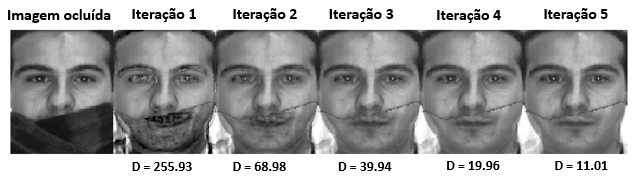
\includegraphics[scale=0.80]{imgs/fast_recursive_pca.png}
\source{Jonas Mendonça Targino, 2018}'
\label{fig:fast_rec_pca}
\end{figure}


\subsection{Fast Robust PCA}
Essa técnica também conhecida como FRPCA \cite{storer2009fast}. Essa técnica possui como base a detecção dos pixels efetivos da imagem parcialmente ocluída usando a combinação de pequenos espaços de faces gerados por amostras de pixels do conjunto de treinamento selecionadas de forma aleatória, de modo que após esse processo a imagem com oclusão é reconstruída a cada iteração a partir da detecção dos pixels efetivos. Na figura \ref{fig:fluxo_frpca} são apresentados o diagrama de fluxo da técnica FRPCA, a qual consiste dos (\textit{i}) processo de treinamento e (\textit{ii}) processo de reconstrução.

\begin{figure}[H]
\centering
\caption{Diagrama de fluxo do processo de reconstrução utilizando a técnica FRPCA}
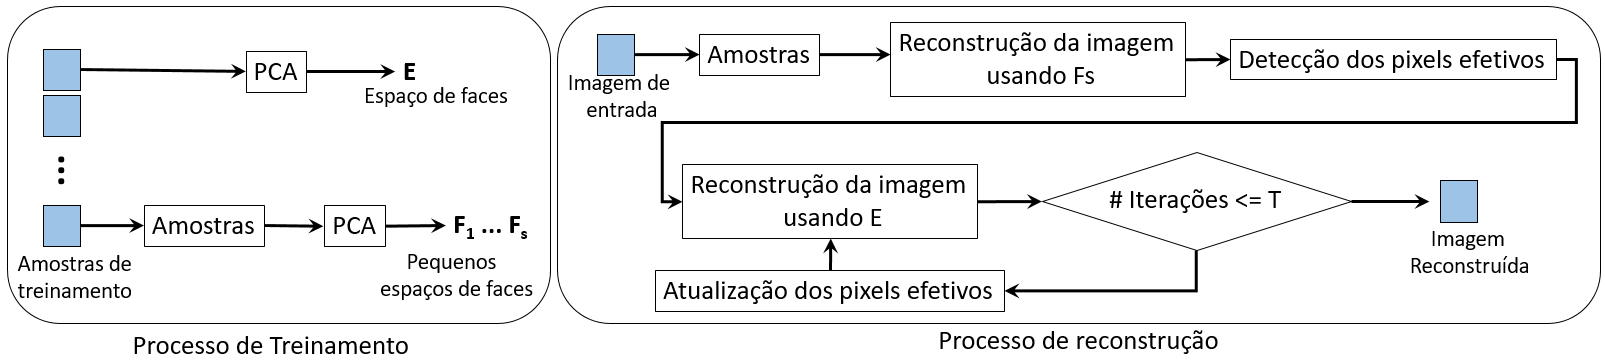
\includegraphics[scale =0.38]{imgs/fluxo_frpca}
\label{fig:fluxo_frpca}
\source{Jonas Mendonça Targino, 2018, adaptada de \citeonline{[37]hosoi2012restoring}}
	\end{figure}

\noindent \textbf{(Processo de treinamento)}

nessa etapa, inicialmente o espaço de faces $E$ é calculado usando todas as imagens do conjunto de treinamento. Logo após $K$ pixels são extraídos de cada imagem do conjunto de treinamento de acordo com $S$ padrões de subamostras. Dessa forma, com as $S$ subamostras do conjunto de treinamento para cada uma delas é gerado seu respectivo espaço de faces, embora esse seja um espaço reduzido, de forma $F_s (s=1,\cdots,S)$. Na figura \ref{fig:frpca} é apresentado o processo de treinamento da técnica FRPCA. 

\begin{figure}[H]
\centering
\caption{Treinamento da técnica Fast Robust PCA}
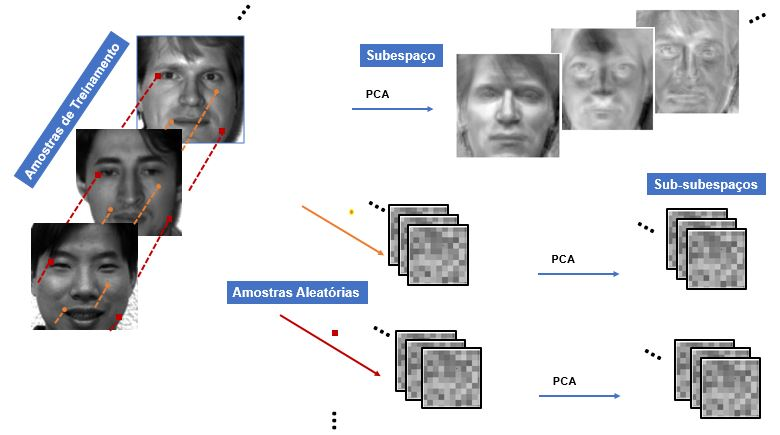
\includegraphics[scale =0.75]{imgs/fastrpca.png}
\label{fig:frpca}
\source{Jonas Mendonça Targino, 2018, adaptada de \citeonline{storer2009fast}}
\end{figure}



\noindent \textbf{(Processo de reconstrução)}

Na segunda etapa o conjunto $\Upsilon_s = \{ s=1, \cdots, S\}$ é gerado para imagem parcialmente ocluída, para $S$ padrões de amostragem aleatória usadas no processo de treinamento. De modo que para $\Upsilon_s$ existe uma imagem reconstruída $\hat{\Upsilon_s}$ que é estimada por meio da correspondência do seu respectivo espaço de faces $F_s$. Então, podemos calcular o erro de reconstrução daquela imagem reconstruída conforme a equação \ref{eq:frpca1}.

\begin{equation}
\label{eq:frpca1}
r_s = \left | \Upsilon_s - \hat{\Upsilon_s} \right |
\end{equation}

Com erro de reconstrução de cada amostra $r_s$ os pixels efetivos são detectados desse modo o pixel \textit{j} da subamostra $\Upsilon_s$ é removido como um pixel faltante se seu erro de reconstrução $r_{sj}$ satisfazer as condições da equação \ref{eq:condi_fprca}

\begin{equation}
\label{eq:condi_fprca}
r_{sj} > \mu_s \overline{r}_s \textrm{   ou  } r_{sj} > \overline{r}
\end{equation}

Em que $\overline{r}_s$ representa a média do erro de reconstrução da amostra $\Upsilon_s$, $\overline{r}$ é a média de todos os erros de reconstrução, $\mu_s$ é um parâmetro que depende  de $\overline{r}_s$. Dessa forma os pixels restantes, ou seja, os candidatos a pixels efetivos, são selecionados a cada iteração, de modo que os $P$ pixels remanescentes são selecionados em ordem ascendente de erro de reconstrução da amostra $r_s$, para que os mesmos possam se tornar pixels efetivos. Então, em cada iteração pontos com baixo erro de reconstrução que foram descartados anteriormente, podem serem inseridos para \textit{\textbf{r}}, e com isso tentar conseguir melhores qualidades de reconstruções.


Desse modo, a imagem ocluída é reconstruída tomando por base a equação \ref{eq:condi_fprca} e dessa forma estimados os $H$ pixels efetivos. Portanto, os pixels faltantes podem ser incluídos como pixels efetivos $H$ a cada iteração a depender de seu erro de reconstrução a cada iteração.  Logo, após $T$ iterações podemos obter a imagem reconstruída. É importante notar que nessa técnica as iterações são repetidas até que o número de pixels efetivos seja reduzido para o número especificado. A figura \ref{fig:frpca_esquema} ilustra o comportamento da técnica FRPCA com seu processo de inclusão dos pixels efetivos a cada iteração.


\begin{figure}[H]
\centering
\caption{FRPCA e seu comportamento frente a detecção da oclusão a cada iteração}
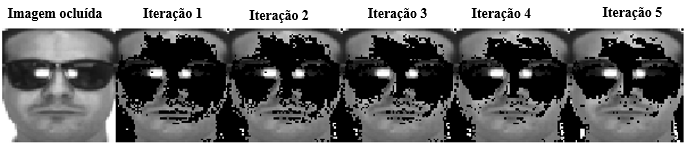
\includegraphics[scale =0.8]{imgs/frpca_esquema.png}
\label{fig:frpca_esquema}
\source{Jonas Mendonça Targino, 2018}
\end{figure}



\subsection{Fisherfaces}

O algoritmo Fisherfaces \cite{belhumeur1997eigenfaces} também conhecido por LDA é uma derivação do PCA, pois utiliza combinações lineares de variáveis independentes para análise se determinada imagem pertence a um dos grupos de imagens. O conjunto de imagens de treinamento da face é composto de várias classes, em que cada classe representa um indivíduo, possibilitando com isso a identificação da classe a que determinada imagem de face pertence. 

A ideia principal do Fisherfaces é encontrar um subespaço que projete os vetores das imagens de cada classe em um único grupo de representação no espaço de faces, de modo que esses grupos estejam tão distantes quanto possível. Logo os vetores resultantes são definidos como Fisherfaces. Este algoritmo encontra uma projeção que minimiza a variação intraclasse como também preserva a variação interclasse.

O Fisherfaces utiliza a matriz \textit{X} para representar as \textit{c} classes de imagens, conforme apresenta a equação \ref{eq:xclasses}. E cada classe possui um conjunto \textit{n} de imagens como podemos perceber na equação \ref{eq:xi}. 

\begin{equation}
X = \{X_1,X_2,X3, \cdots ,X_c\}
\label{eq:xclasses}
\end{equation}


\begin{equation}
X_i = \{x_1,x_2,x_3, \cdots ,x_n\}
\label{eq:xi}
\end{equation}

Com isso, as matrizes \textit{$S_B$}, \textit{$S_W$} podem ser calculados de acordo com as equações \ref{eq:SB} e \ref{eq:SW} respectivamente.

\begin{equation}
S_B = \sum_{i=1}^{c}N_i(\mu_i - \mu)(\mu_i - \mu)'
\label{eq:SB}
\end{equation}

\begin{equation}
S_W = \sum_{i=1}^{c}\sum_{x_j \epsilon X_i}^{ }  (x_j - \mu_i) (x_j - \mu_i)'
\label{eq:SW}
\end{equation}

Nas equações \ref{eq:mediageral} e \ref{eq:mediaDaClasse} são apresentadas respectivamente  a média geral $\mu$ e a média de cada classe $\mu_i$.

\begin{equation}
\mu = \frac{1}{M}\sum_{i=1}^{M}x_i
\label{eq:mediageral}
\end{equation}

\begin{equation}
\mu_i = \frac{1}{\left | X_i \right |} \sum_{x_j \epsilon X_i }^{ }x_j
\label{eq:mediaDaClasse}
\end{equation}

O algoritmo Fisherfaces clássico cria uma projeção $\Phi$ com iniciativas a maximizar os critérios de separabilidade entre as \textit{C} classes.
\begin{equation}
\Phi_{opcional} = argmax_\Phi \frac{\Phi^T S_B \Phi}{\Phi^TS_\Phi \Phi}
\end{equation}

Entretanto essa solução apresentava-se consideravelmente custosa, mediante isso, \citeonline{belhumeur1997eigenfaces} apresentou uma solução com maior viabilidade computacional, resolvendo o problema com o auxílio dos autovalores:

\begin{equation}
S_Bv_i  =  \lambda_i S_\Phi \cdot v_i  
\end{equation}

\begin{equation}
S_\Phi^{-1}S_B v_i = \lambda_iv_i 
\end{equation}

Todavia, surgiu um problema de modo que \textit{$S_\Phi$} é no máximo (\textit{N - C}) com \textit{N} amostras e \textit{C} classes. Levando essa justificativa para o contexto de reconhecimento de imagens, normalmente  o número de imagens é muito menor que sua dimensão, de modo que a matriz $S_\Phi$ torna-se singular. Diante dessa questão uma nova solução foi proposta por \citeonline{belhumeur1997eigenfaces}, em que foi aplicado o  PCA sobre as amostras e os projetou no espaço ($N - C$) dimensional, e logo em seguida os associou com o LDA, como pode ser visto nas equações \ref{eq:wpca} e \ref{eq:wfld}.

\begin{equation}
\Phi_{pca} = argmax_\Phi\left |\Phi^TS_T\Phi  \right|
\label{eq:wpca}
\end{equation}

\begin{equation}
\Phi_{lda} = argmax_\Phi \frac{\left |\Phi^T\Phi_{pca}^TS_B\Phi_{pca}\Phi \right |}{ \left| \Phi^T\Phi_{pca}^TS_\Phi\Phi_{pca}\Phi \right |}   
\label{eq:wfld}
\end{equation}

Logo a matriz de transformação $\Phi$, projeta uma amostra no espaço (C-1) dimensional, esse processo pode ser visualizado pela equação \ref{eq:wfinal}.

\begin{equation}
\Phi = \Phi_{lda}^T\Phi_{pca}^T
\label{eq:wfinal}
\end{equation}

Na figura \ref{fig:fisherfaces} são apresentados 10 fisherfaces da base dados AR, sendo calculado o PCA com 95\% de percentual de representatividade do conjunto.

\begin{figure}[H]
\centering
\caption{Exemplos de 10 fisherfaces da base de dados \textit{AR}}
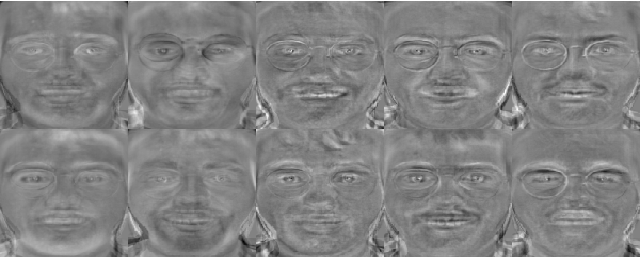
\includegraphics[scale = 0.75]{imgs3/fisherfaces.png}
\source{Jonas Mendonça Targino, 2018}
\label{fig:fisherfaces}
\end{figure}






\section{Técnicas de reconstrução baseadas em modelo}
As técnicas baseadas em modelo possuem como princípio básico a construção de um modelo computacional que represente o conjunto de faces, sem a necessidade de projetar a face parcialmente ocluída em um subespaço. 



\subsection{Representação Esparsa com Grafo de Poisson}
\label{sub:RS_GP}


Essa técnica proposta por \citeonline{[25]deng2011graph} é baseada em um grafo espectral para reconstrução de faces. Sendo composta de três processos principais: (\textit{i}) aplicação da Representação Esparsa na parte não ocluída, com iniciativa a descobrir quais indivíduos da base de treinamento possuem tal parte com maior grau de semelhança; (\textit{ii}) mineração da imagem com maior valor de alfa; e (\textit{iii}) aplicação do Grafo de Poisson com formulação da matriz Laplaciana para descoberta dos pixels ocluídos.


A Representação Esparsa possui como principal objetivo identificar faces com similaridades perante um determinado conjunto, tomando para o contexto de faces ocluídas, dada uma face parcialmente ocluída é aplicada a Representação Esparsa como forma de analisar quais imagens de face presentes no conjunto de treinamento possuem maior semelhança. Essa semelhança é obtida por meio da combinação linear de todas as imagens de face e um vetor de erros no nível de pixel. Um dos primeiros trabalhos a utilizar SRC para o reconhecimento de faces ocluídas foi proposto por \citeonline{Wright_2009}.

Estudos realizados por \citeonline{[32]wright2009robust,yang2010metaface,zhang2010dimensionality} indicam que SRC possibilita obter performances consideráveis perante a tarefa de reconhecimento de faces parcialmente ocluídas. 

Na SRC, uma face ocluída parcialmente é vista como um sinal. E graças ao uso dela como sinal é possível obter sua SRC usando as imagens presentes no conjunto de treinamento. Dessa forma $\Upsilon$ é a imagem parcialmente ocluída representada como um sinal, de modo que a matriz de treinamento é da forma $\Gamma$ = $[I_1,I_2,\cdots, I_M]$, contendo $M$ imagens. E $\mathbf{x}$ representa o vetor de coeficientes de correlação. Logo, na equação \ref{eq:SR} podemos perceber a estrutura de uma representação Esparsa.

\begin{equation}
\Upsilon = \alpha_1I_1 + \alpha_2I_2 + \cdots + \alpha_MI_M = \mathbf{\Gamma} \cdot \mathbf{x}
\label{eq:SR}
\end{equation}

O vetor de coeficientes de correlação de forma $\mathbf{x} = [\alpha_1,\alpha_2, \cdots, \alpha_M]$ possuem importância significativa para a imagem parcialmente ocluída, visto que o valor de $\alpha_i$ no intervalo [0,1] representa a semelhança entre as imagens $I_i$ e $y$. Logo, quanto maior o valor de $\alpha_i$ maior sua correlação com a imagem parcialmente ocluída. Vale a pena notar que o vetor $\mathbf{x}$ é esparso, ou seja, a maioria de seus valores são próximos de zero. 

Segundo \citeonline{[32]wright2009robust} com o vetor esparso apenas as imagens com maiores de alfa realizaram contribuições significativas perante a imagem parcialmente ocluída $y$. Dessa forma, no contexto de faces parcialmente ocluídas para obtermos valores de alfa com maiores valores de confiança devemos realizar a comparação dos pixels não ocluídos da imagem $y$ com os pixels não ocluídos das imagens do conjunto de treinamento $\Gamma$.

Logo a SRC pode ser vista como uma equação linear, da forma $\Upsilon = \mathbf{\Gamma} \cdot \mathbf{x}$, sujeita ao problema otimização da equação \ref{eq:sr1}.

\begin{equation}
\label{eq:sr1}
(l^0): \hat{x_0} = argmin\left \| x \right \|_0  x \mapsto  \Gamma \cdot \mathbf{x} = \Upsilon
\end{equation}

Mediante esse problema de otimização, o trabalho de \citeonline{chen2001atomic} e \citeonline{huang2010fast} apresentam soluções que resolvem a equação \ref{eq:minsr} em tempo polinomial. Entretanto neste trabalho adotou-se a formulação proposta por \citeonline{huang2010fast}, a qual encontra-se disponível publicamente \footnote{http://faculty.ucmerced.edu/mhyang/papers/cvpr10a.pdf}.

\begin{equation}
\label{eq:minsr}
(l^1): \hat{x_1} = argmin\left \| x \right \|_1  x \mapsto  \Gamma \cdot \mathbf{x} = \Upsilon
\end{equation}



Após o retorno dos alfas pela SRC são utilizadas as 20 imagens do conjunto de treinamento com maiores valores de $\alpha$, mediante esse processo essas imagens retornadas são analisadas com base na métrica SSD (do inglês: \textit{Sum Square Distance}) com finalidades a encontrar a imagem do conjunto de treinamento com maior semelhança dos pixels de borda da parte ocluída. Logo, é definida uma quantidade $q$ de pixels de borda a serem adicionadas nas regiões de borda dos pixels ocluídos e com isso analisados os respectivos pixels nas imagens do conjunto de treinamento.

Um dos motivos de utilizar a métrica SSD para analisar a face com maior correlação com a imagem parcialmente ocluída é que a SRC necessita de outras métricas para dar suporte a sua classificação quando apresentada a tipos de dados com muita variação de ruído. Visto que utilizar o retorno com maior valor de alfa nem sempre implica em realizar uma correta classificação, daí surgindo a necessidade de utilizar o SSD.  O emprego do SSD torna-se necessário visto que em muitos cenários práticos de reconhecimento facial, as amostras de treinamento de cada indivíduo são muitas vezes insuficientes, no caso extremo somente uma face de cada indivíduo pode estar disponível, dessa forma dando suporte a classificação realizada pela SRC.


Na figura \ref{fig:ssd} ilustra-se a oclusão parcial, a região $J$ significa os pixels de borda, nesse caso utilizando uma região de pixels de borda $q$ igual a 10 pixels. Enquanto $F$ representa a imagem ocluída. Logo para analisar qual das 20 imagens retornadas da SRC possuem maiores semelhanças dos pixels de borda são utilizados os pixels da região $J$.

\begin{figure}[H]
\centering
\caption{Parte ocluída e  aplicação das bordas na região ocluída, e por último a topologia do grafo de Poisson}
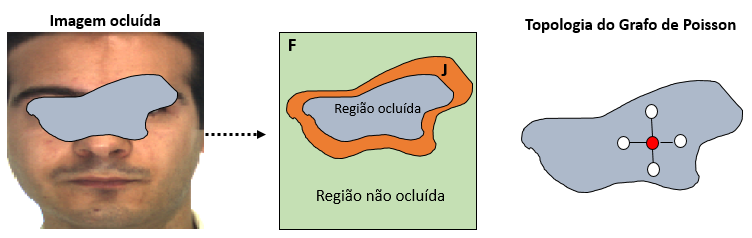
\includegraphics[scale = 0.8]{imgs/ssd}
\source{Jonas Mendonça Targino, 2018}
\label{fig:ssd}
\end{figure}

A área $J$ pode ser obtida com a aplicação de filtros morfológicos de erosão na máscara binária de oclusão. Nesse trabalho foi aplicada 10 vezes seguidas tal filtro morfológico na máscara de modo a possuir uma região $J$ que circunda a área ocluída da imagem.  
 
O cálculo do SSD pode ser resolvido com o auxílio da equação \ref{eq:ssd}, em que SR representa as 20 imagens retornadas pela representação esparsa. 

\begin{equation}
SSD(x_0) = \sum_{x\in F }J(x)(F(x) - SR(x_0 - x))^2 
\label{eq:ssd}
\end{equation}

Logo o Grafo realiza a reconstrução da imagem parcialmente ocluída tomando por base a imagem retornada pela SRC com menor SSD, ou seja, com maior similaridade dos pixels de borda da oclusão.

O grafo de Poisson para reconstrução de faces proposto por \citeonline{[25]deng2011graph},  possui como base a teoria de reconstrução da face via modelos gráficos de modo que cada pixel é representado por um nó no grafo, e os pixels não rotulados (ocluídos) são rotulados após a resolução de um sistema linear.

O grafo de Poisson possui como base um grafo $G = \{V,E\}$, com vértices $v$ $\in$ $ V$ e arestas $e$ $\in$ $E$ $\subseteq$ $V$ x $V$, em que existe uma matriz binária $W$ que indica a relação entre os nós.

Para reconstrução da imagem são utilizados dois grafos  $G_{no}$ e $G_o$   de mesma topologia, de modo que $G_{no}$ representa o grafo gerado pela imagem do treinamento com menor SSD, lembrando que esse grafo possui todos os seus nós rotulados, visto que não apresenta oclusão, enquanto $G_o$ é o grafo gerado pela imagem de consulta a qual possui alguns nós rotulados (pixels não ocluídos) e outros não rotulados (pixels ocluídos).


O objetivo desse grafo é tentar obter os rótulos faltantes em $G_o$ para tentar reconstruir a imagem original. Para atingir tal objetivo deve-se realizar algumas operações com os dois grafos gerados, umas das primeiras operações a ser realizada é calcular a diferença dos dois grafos, podendo ser obtida pela forma $\Delta G = G_o - \kappa G_{no}$, de modo que $\kappa$ é um parâmetro no intervalo [0,1],  responsável por controlar o grau de participação de $G_{no}$ na tarefa de reconstrução dos nós não rotulados de $G_o$. 

Tendo em vista o domínio Euclideano, a equação Laplaciana pode ser visualizada com o auxílio da equação \ref{eq:delta}, o operador de Laplace é definido por $\Delta^2$.

\begin{equation}
\Delta^2(G_o - \kappa G_{no}) = 0
\label{eq:delta}
\end{equation}

Entretanto, o Grafo de Poisson é implementado tendo como base o domínio gráfico que pode ser representado pela matriz Laplaciana $\textbf{L}$ na teoria dos grafos espectrais, como demonstra a equação \ref{eq:teoria_dos_grafos}. 

\begin{equation}
\textbf{L} = D - W
\label{eq:teoria_dos_grafos}
\end{equation}

De modo que $D= diag(\sum_j W_{ij})$ em que $D$ é chamado de grau da matriz na teoria espectral dos grafos e $W$ é a matriz de pesos com entradas $W_{ij}$, $W$ representa a máscara de oclusão da imagem de consulta como uma matriz simétrica que representa a correlação entre os nós no grafo, contendo o valor 1 nos pixels não ocluidos e 0 nos pixels ocluídos. Logo a equação final para o cálculo de $G_o$ pode ser escrita  na equação \ref{eq:equacao_final}.

\begin{equation}
\textbf{L} G_o =  \kappa \textbf{L} G_{no}
\label{eq:equacao_final}
\end{equation}

 A figura \ref{fig:estrutura_src_gp} ilustra detalhadamente o processo necessário para realizar a reconstrução com Grafo de Poisson.

\begin{figure}[H]
\centering
\caption{Estrutura da técnica SRC com Grafo de Poisson}
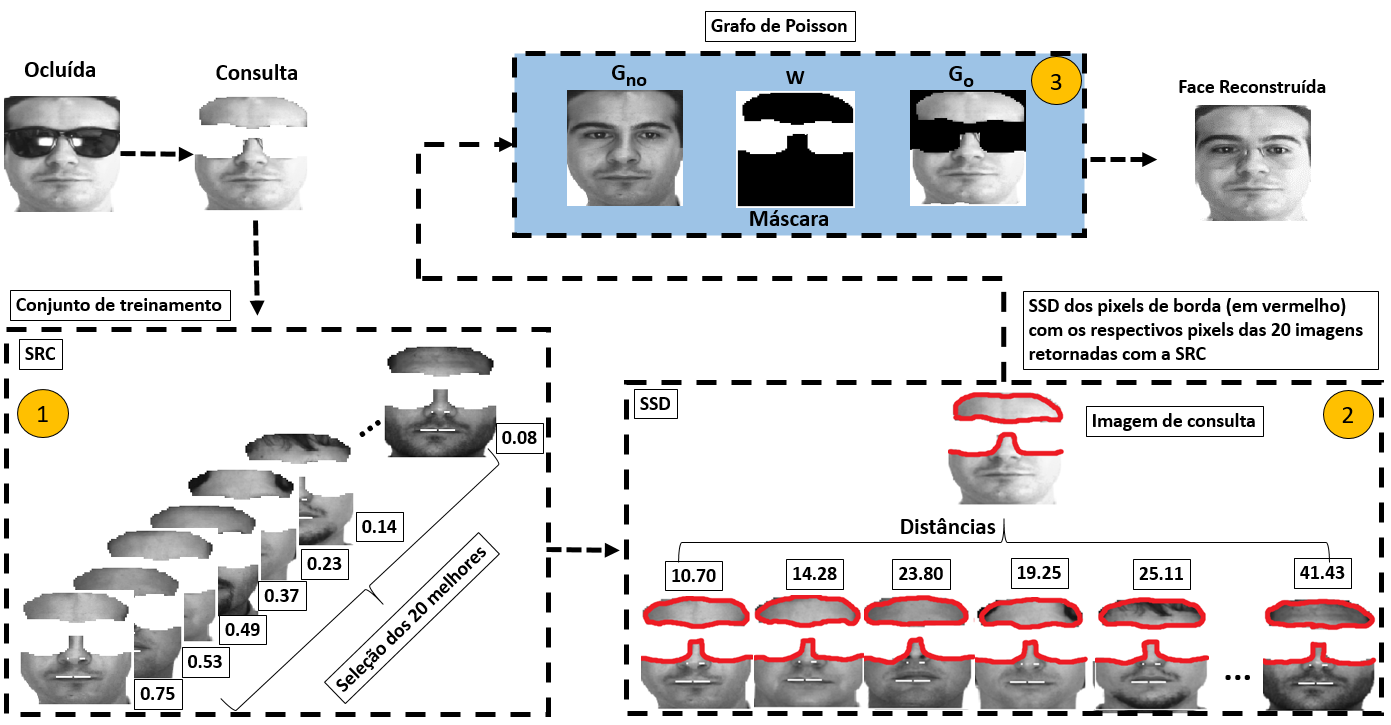
\includegraphics[scale = 0.40]{imgs4/estrutura/estrutura_src_gp}
\source{Jonas Mendonça Targino, 2018}
\label{fig:estrutura_src_gp}
\end{figure}

Logo para descobrirmos os pixels ocluídos temos que resolver o sistema que pode ser decomposto com o auxílio da formulação abaixo.



\[
\begin{matrix}

\\
L = D - W \\
L = diag\left [  \sum_{j}W_{ij} \right ] - W\\
\\
= \begin{bmatrix}
\begin{matrix}
\sum_jW_{1j} &    & \\
  &  \sum_jW_{2j} &  & \\
  &  & \ddots & \\
  &          & & \sum_jW_{nj} 
\end{matrix}
\end{bmatrix}

- W
\\[6pt]
\\[6pt]
%\\[6pt]

\end{matrix}
\]

\textit{Dessa maneira a matriz Laplaciana do grafo com 4 conexões é da forma:} %\\[6pt] \\[6pt]

\[
\begin{matrix}

\\
\textbf{L}G_{no}=\begin{bmatrix}
\begin{matrix}
4 &  -1  & -1 &-1 &-1 &\ldots 0\\
-1  &  4 & -1 &-1 &-1 &\ldots  0\\
-1  &-1  &4   &-1 &-1 &\ldots0\\
-1  &-1  &-1   &4 &-1 &\ldots0\\
\vdots & \vdots & \ddots &  &\ddots\\
0  &   \ldots&-1 & -1 &-1    &4
\end{matrix}
\end{bmatrix}
.
\begin{bmatrix}
\begin{matrix}
G_{no_1} \\
G_{no_2}  \\
G_{no_3} \\
$\vdots$\\
G_{no_{(n-1)}} \\
G_{no_n}  \\
\end{matrix}
\end{bmatrix}
\\%[6pt]
%\\[6pt]
\textit{Com isso, chegamos a resolução do sistema geral, pela forma:} 
\\%[2pt]
%\\
\textbf{L}G_{no} = \kappa\textbf{ L}G{o}
\end{matrix}
\]

 Logo após a descoberta do sistema temos que apenas substituir os pixels ocluídos na imagem parcialmente ocluída pelos pixels retornados pela resolução do sistema linear da matriz laplaciana.




\section{Considerações finais do capítulo}

Neste capítulo foram apresentadas as técnicas para detecção e reconstrução das oclusões parciais, de modo que foram implementadas três técnicas para detecção da oclusão, dessas três a que apresentou melhores segmentações da área ocluída foi a técnica BMA. Enquanto das técnicas de reconstrução foram apresentadas oito técnicas, sete baseadas em subespaço e uma baseada em modelo.

